\chapter{Variable Range Hopping}		% chapter 1
\label{theorychap}

\section{History}
In 1937, Nevill Mott and Rudolf Peierls explained why some materials which should have been conductors, acted as insulators. This was due to electron-electron interactions, which is not taken into account in band theory ~\cite{mott72}. From there, Miller and Abrahams proposed a network resistor model which Efros and Schklovskii built on ~\cite{efros75}. Because of the dynamic complexity of even a small system (a 10 by 10 system can have $2^{100}$ configurations) simulations are a large part of modern electron hopping studies ~\cite{kirkengen09}. The theory has gotten more consise over time. For the sake of simulation, much of it can be compressed into equation~\ref{probability}.

\section{Jump Probability}

In order to calculate were the electron will jump, we must first find the probability of each jump site. Our main equation involved is as follows:
\begin{eqnarray}
P_{ij} = \exp (-2\alpha R_{ij} -  E_{ij}/kT)
\label{probability}
\end{eqnarray}

where $k$ is the Boltzmann constant, $R_{ij}$ is the distance between cells, $E_{ij}$ is the energy change of the system if a particle were to move from i to j, and T is the temperature of the system. $E_{ij}$ has various inputs which vary in energy scale.
\begin{eqnarray}
E_{ij} =  \triangle U_{ij} e^2/a\kappa_1  + e f_i \triangle V_{ij} + f_i  \triangle \mu_{ij} + f_i (eV) \triangle x_{ij} 
\label{deltaE}
\end{eqnarray}
where $i$ refers to the starting site index and $j$ refers to the target site index,  $f$ is the occupation of a site, $a$ is the size of the granule, $\kappa_1$ is the intra-granule dielectric constant, $\mu$ is the substrate potential, $V_{ij} = \sum_{n=1}^{N} e^2/\kappa_2 r_{n}$ is the local potential from the rest of the particles, $\kappa_2$ is the inter-granule dielectric constant, $\triangle x$ is the component of r in the direction of eV , and $eV$ is an externally applied voltage. $\triangle U_{ij}$ is -1 if electrons stacked, 1 if electrons de-stacked, and 0 otherwise. The first two components of equation ~\ref{deltaE} together constitute the electrostatic component of this system. The most powerful is the Coulomb blockade. This introduces a large penalty into the probability of an electron occupying the same site as another electron. If the site at which an electron can travel to is empty, the chances of transport are higher than if the site is filled ~\cite{glazman05}. There is also a contribution from the substrate. There is an inherent randomness in the potential at different lattice sites and that is where this comes in. This energy landscape somewhat randomizes starting energies and can fill in as electron donor. There is a general electric potential which will try to get the electrons to space out evenly in the substrate (periodic boundary conditions). Finally there is a current portion which if a voltage bias is applied on the left and right sides of the system, then the probability of electrons hopping with that bias is increased ~\cite{aharony92}. The exponential term is artificially limited below 0 to keep the electron hop ranges realistic. Analytically, equation~\ref{probability} can be maximized to find the most common jump distance (take the derivative with respect to r and set equal to 0). In our case, there are 2 problems with this approach. First, we are more interested in the average jump distance which need not be the maximum. Second, The analytical approach assumes a continuous system, where in reality it is a discrete number of interacting points. There are a few nuances in the theory that need to be adressed.
\subsection{Mott vs. Effros-Schklovskii}
While the approach to describe physical systems by Mott vs Effros-Schklovskii (ES) theory are similar, there are a few key differences in the details. First, The localization parameters are different due to differences in the density of states. The localization is temperature dependent in the ES system. This is because ES considered the situation where if an electron tries to tunnel, It must leave an electron hole behind. This enhanced requirement for the energy means that at low temperatures, the density of states at the Fermi level vanishes ~\cite{joung}. The resistivity for the Mott system ends up being related to the temperature as

\begin{eqnarray}
\ln(\rho) \approx (T_o / T)^{1/4} ,
\label{fourth}
\end{eqnarray}
where $\rho$ is the resistivity and $T$ is the temperature. Meanwhile, in the ES system we have
\begin{eqnarray}
\ln(\rho) \approx (T_o / T)^{1/2}.
\label{half}
\end{eqnarray}
The Mott resistance comes from $\delta E = \alpha_1 / g r_{ij}^3 $, where $\alpha_i$ are prefactors of order unity. The ES resistance comes from the usual Coulomb blockade term $\delta E = \alpha_2 e^2 / \kappa r_{ij}$ ~\cite{aharony92}. The Differences can be summarized in a single plot ~\ref{MvsES} ~\cite{Liu10}.

\begin{figure}[htbp]
\begin{center}
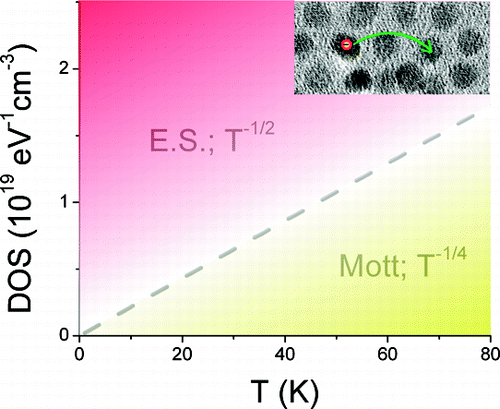
\includegraphics[scale=.50]{MottvsES.png}
\caption{Density of states vs Temperature. This plot describes the interface between ES and Mott transmission of electrons. (Graph courtesy of Heng Liu)}
\label{MvsES}
\end{center}
\end{figure}

\subsection{Coulomb Glass vs Artificial Nanosolids}
Coulomb glasses are the original substrate on which the ES model of electron conduction was based. The "glass" in coulomb glass refers to a phase in which electron-electron interactions impair conduction and dynamics become slow, like the flow of a glass~\cite{ortuno04}. Artificial nanosolids are arrays of granules which have a higher intra-granule conduction than a inter-granule conduction. The differences begin at the density of states. In artificial nanosolids, the density of states can be more creative. By changing the size of the granule, and the material it is made out of (metal, insulator, superconductor) the amount of available electron slots per site (and the energy of each slot) can be chosen. There are two energy scales for each grain. $\delta$ is the mean level spacing. $E_c$, the energy required to pack on one more electron onto a site is on the order of 3000 Kelvin ~\cite{glatz08} .The distances are also different. For coulomb glasses, the distances are basically the inter-atomic distances. There we are basically talking about electron jumps between atoms on a crystal lattice. As the name suggests, in artificial nanosolids the distances are arbitrary. For typical artificial nanosolid applications, we are in the nanometer to tens of nanometers range~\cite{beloborodov05}. While the general electric potential plays a role in both systems, It plays a bigger role in the coulomb glass since the scales are smaller and the electric potential scales as $1/r$.

\subsection{Inelastic vs. Elastic tunneling}
As well as blocking each other, electrons also can impart energy onto each other which may result in an electron being dislodged. This is referred to as inelastic co-tunneling. If instead the electron tunnels or otherwise travels without dislodging, it is referred to as elastic co-tunneling (see fig. ~\ref{inelasticvselastic}). For low to medium temperatures, the main tunneling mechanism will be elastic. At higher temperatures, we expect a transition to in-elastic tunneling~\cite{Glazman05}.

\begin{figure}[htbp]
\begin{center}
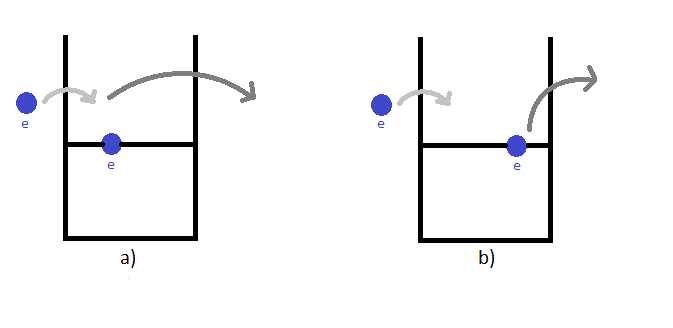
\includegraphics[scale=.50]{inelasticvselastic.png}
\caption{a) elastic transmission of electrons. b) inelastic transmission of electrons.}
\label{inelasticvselastic}
\end{center}
\end{figure}

\subsection{Temperature}

Temperature-dependent phase transitions are scattered throughout the spectrum and so it is important to specify at which temperatures we are working with. At temperatures lower than the Neel temperature, We encounter the first transition called "Mott-Heisenberg". At these low temperatures, the magnetic fields of the electrons have a chance to couple into anti-ferromagnetic pairs. Also, During tunneling events, electrons will avoid atoms which are occupied with other electrons of similar spins as sharing an atom would require an increase in energy compared to one of opposite spin ~\cite{Gebhard03}. At medium temperatures, we have a transition between elastic and inelastic. In order for an electron to land on an occupied site it must have enough energy to overcome the Coulomb blockade. This is only possible if it was given enough kinetic energy from a phonon (sufficient thermal energy). As the temperature is increased, electrons can begin stacking. Once an electron stacks onto another electron, Coulomb repulsion guarantees that either electron will quickly move on~\cite{Glazman05}. At much higher temperatures, the system starts to have enough free thermal energy to exceed the coulomb blockade energy. That is, the energy required to stack 2 electrons in the same quantum dot. This yields a crossover temperature which was discussed during our comparison of ES vs Mott systems ~\cite{aharony92}. Depending on the density of states, there will eventually be higher energy states on which to pack on electrons. For our purposes, we will stay in between these two systems. Our temperatures will be high enough that magnetic moments can be ignored, yet low enough that the maximum number of electrons allowed on the same quantum dot will be two.

\subsection{Density of States}
There are many methods of characterizing the energy of an electron. One of these is the density of states. This is a histogram of the energies that electrons can be in. For example in ~\ref{moundDoS}, there are many electrons at a relatively low energy and the number of electrons with higher energies decreases with energy. In ~\ref{crystalDoS} there is only one energy option for electrons. We see two peaks because the holes act as particles in that the system requires energy to move those as well. The value on the x axis is the energy required to fill or empty each hole or particle respectively. By knowing the shape of the density of states, one can discern important intricacies of a system. These can include the energy scales, the relaxedness, and the bandgap of a system. The typical kinetic energy of an electron in a fermi glass is $E = E_o + \frac{(\hbar k)^2} {2m}$. If one follows through the math, the dispersion relation ends up as $D_n(E) = \frac {nc_n} {p c^{n/p}_k} (E- E_o)^{n/p-1}$ ~\cite{Kittel96}. If the particle distribution is symmetric (same amount of electrons as holes) then the density of states will be symmetric, as long as the system is relaxed.

\begin{figure}[htbp]
\begin{center}
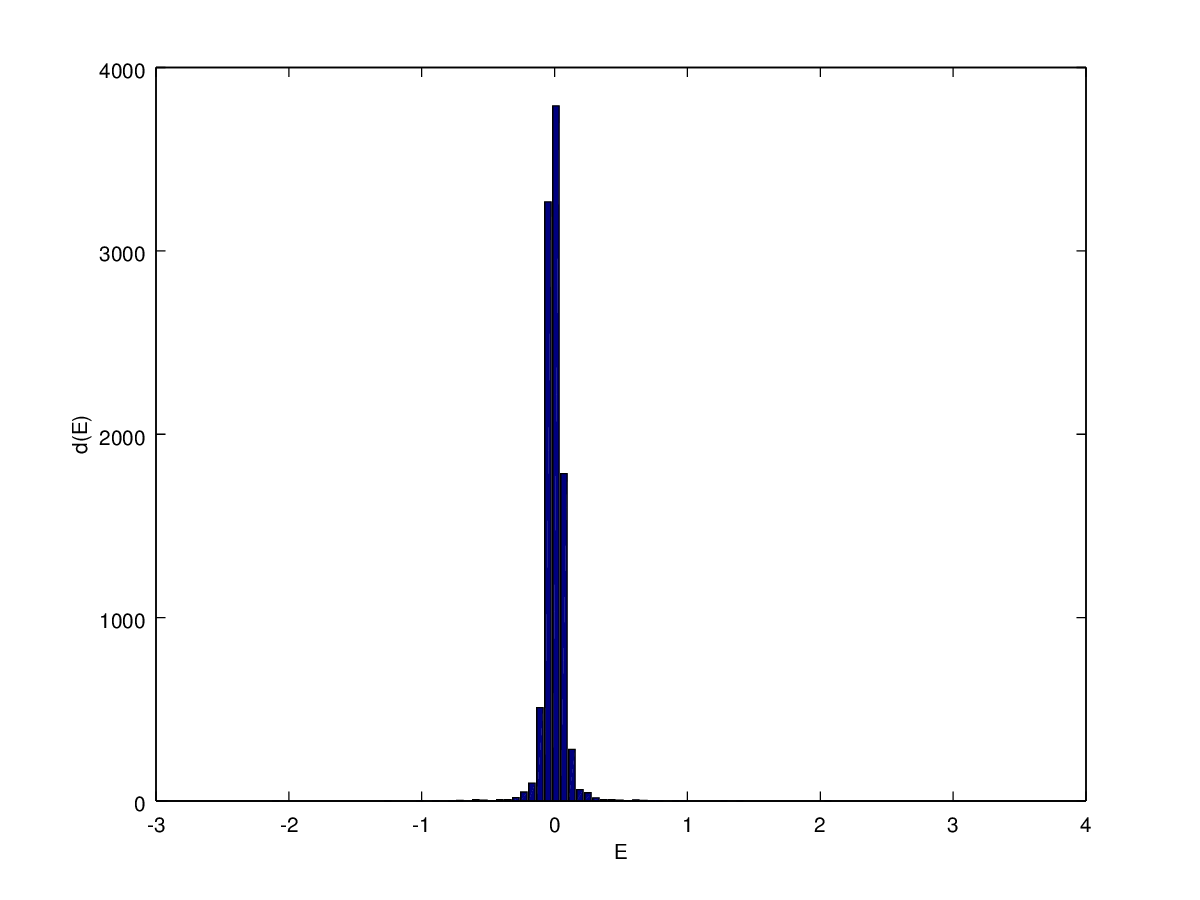
\includegraphics[scale=.50]{veryCloseDos.png}
\caption{The density of states for a system with a high amount of randomness in the energy.}
\label{moundDoS}
\end{center}
\end{figure}

\begin{figure}[htbp]
\begin{center}
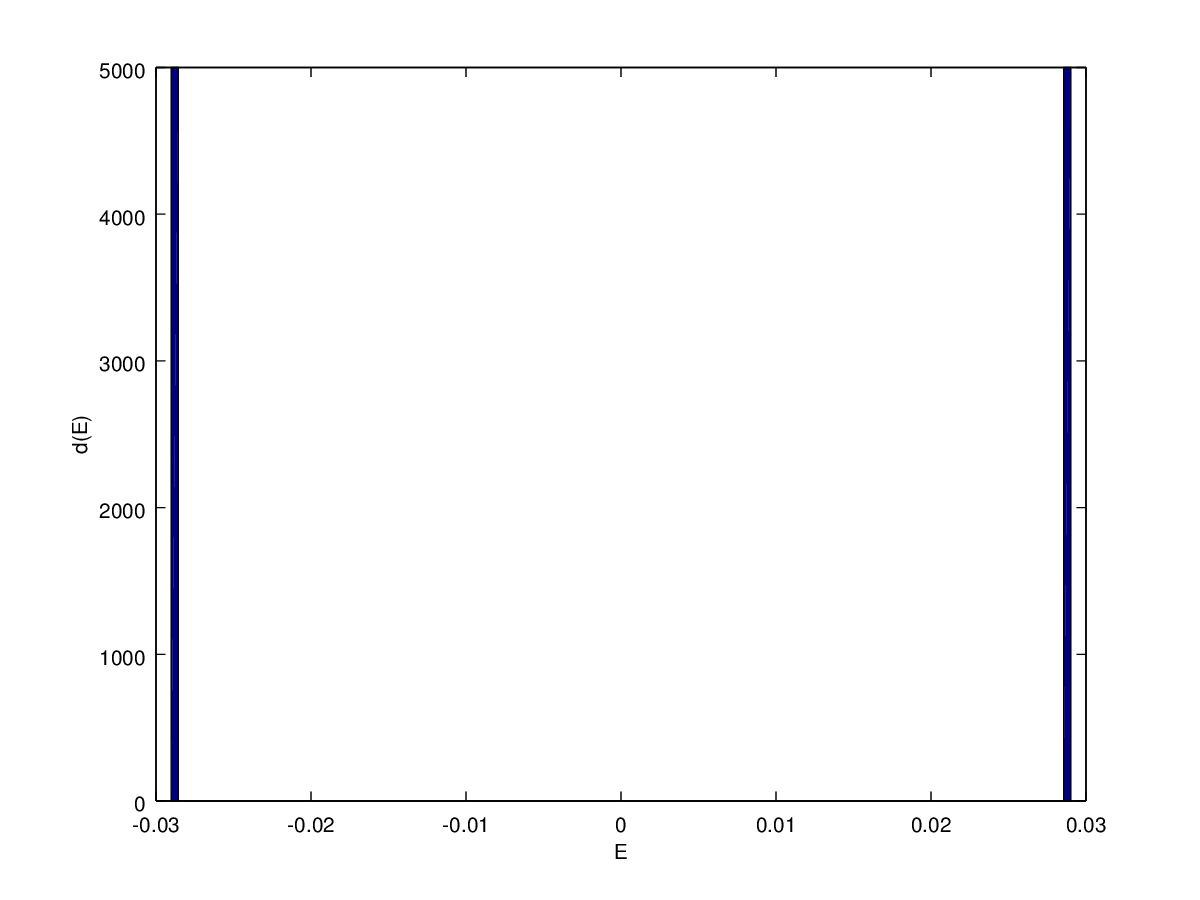
\includegraphics[scale=.50]{splitDos.png}
\caption{A low entropy system (Wigner crystal).}
\label{crystalDoS}
\end{center}
\end{figure}




